%
% detektor.tex -- Schaltbild Detektorradio
%
% (c) 2018 Prof Dr Andreas Müller, Hochschule Rapperswil
%
\documentclass[tikz,12pt]{standalone}
\usepackage{times}
\usepackage{amsmath}
\usepackage{txfonts}
\usepackage[utf8]{inputenc}
\usepackage{graphics}
\usepackage{color}
\usepackage{pifont}
\usepackage{circuitikz}
\usetikzlibrary{arrows,intersections,math,calc}
\begin{document}

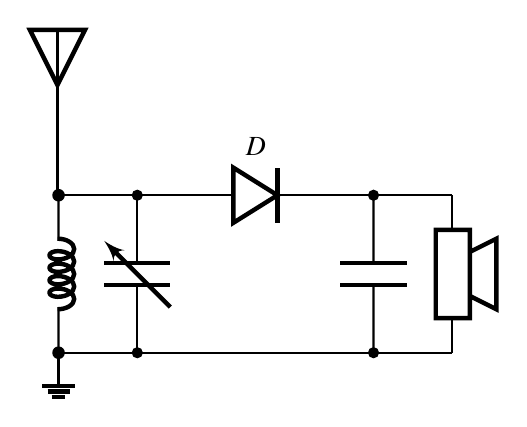
\begin{tikzpicture}[>=latex,thick]

\draw (1,2) to[L, n=l1] (1,0);
\draw (2,0) to[vC, n=l1, *-*] (2,2);
\draw (1,2) -- (2,2);
\draw (1,0) -- (6,0);
\draw (2,2) to[D=$D$] (5,2);
\draw (5,2) -- (6,2);
\draw (5,0) to[C, *-*] (5,2);
\draw (6,2) to[loudspeaker] (6,0);
\node[antenna] at (1,2) {};
\fill (1,2) circle[radius=0.08];
\fill (1,0) circle[radius=0.08];
\node[ground] at (1,0) {};

\end{tikzpicture}

\end{document}

